\chapter{Design\label{chap:design}}
In this chapter, I will talk in-depth the elements that I created during this project and how they interconnect. You can expect a design charts showcasing high-level overview, alongside dividing it onto smaller subsections - each independent and capable of running on its own. I will also explain novel approaches such as verifying the authenticity of the connecting clients, data model stored on a blockchain or how the connection is secured from man-in-the-middle attacks through TLS encryption.

\section{Architecture}
This section includes the diagram of them system and two sample workflows demonstrating how packets are flowing through the framework.
\subsection{Overview}
\begin{figure}[h]
    \centering
    \makebox[\textwidth][c]{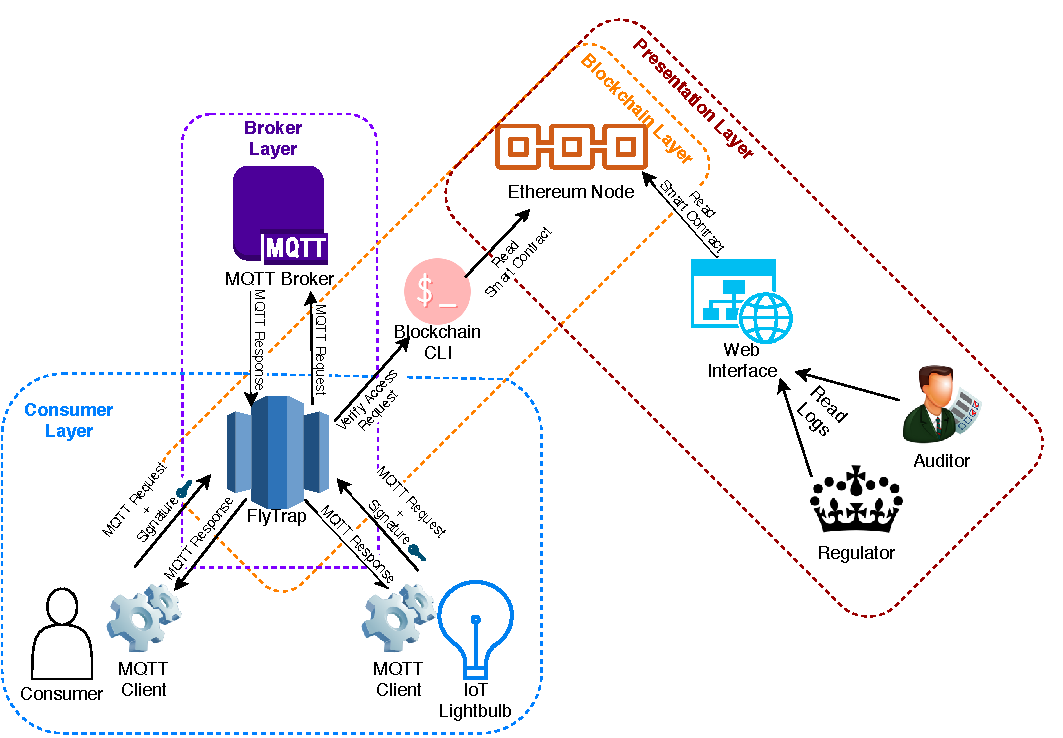
\includegraphics[width=1.2\textwidth]{flytrap}}
    \caption{FlyTrap high-level architecture overview}
    \label{fig:flytrap}
\end{figure}
Figure \ref{fig:flytrap} presents an overview of the system, decomposing it onto four layers, each responsible for a different part of the framework. It also demonstrates how those layers are coupled and the direction of data flowing between them.

To overview, we can distinguish four layers:
\begin{description}
    \item[Consumer Layer] - layer responsible for interacting with end-devices. To them, FlyTrap should be indistinguishable from normal MQTT broker and thus accepts/responds with MQTT v5.0 compliant TCP/TLS packets. In order to compute the signature and attach it to 
    \item[Consumer Layer] - layer where FlyTrap acts like a client for MQTT Broker. Similar to Consumer Layer, all packets sent by FlyTrap need to be compliant with MQTT standard in order to receive valid responses from the broker. In this situation, used MQTT broker is not relevant - as long as it implements the standard.
    \item[Blockchain Layer] - layer in which FlyTrap performs communication with the Ethereum node through a separate CLI. FlyTrap is capable of either reading the past contracts/transactions or submitting new ones. That is also the only way to amend the state of the blockchain - given the private master key has remained secret.
    \item[Presentation Layer] - layer used by FlyTrap's end-users which allows to overview the state of the blockchain in a user-friendly way, easily extracting most relevant information such as recent access changes or audit trail for major operations on the chain.
\end{description}


\subsection{Sample successful PUBLISH workflow}
To provide further context, figure \ref{fig:workflow_success} provides an example process in which a client wants to publish a message to the broker and is successful in doing so. The diagram shows step-by-step logic performed at each stage of the connection, until client receives the response. I'll annotate each step with either \textbf{BL} - Blockchain Layer, \textbf{CL} - Consumer Layer or \textbf{ML} - MQTT Broker Layer to signify on which layer this step is taking place on.
\begin{figure}[h]
    \centering
    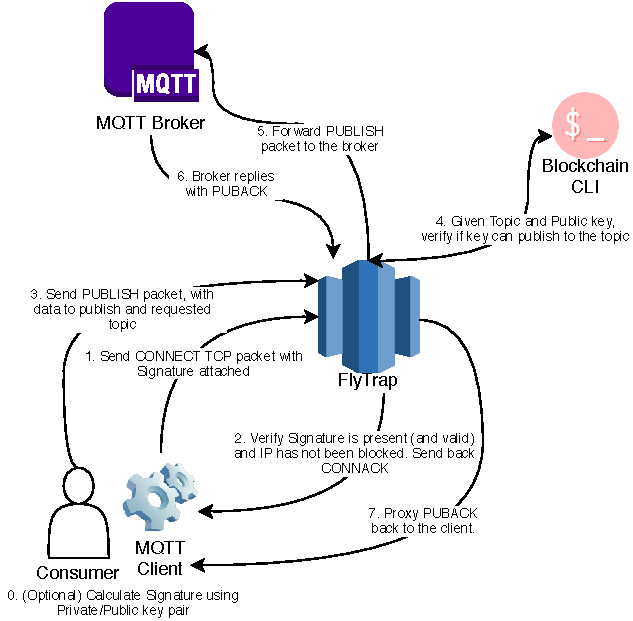
\includegraphics[width=0.8\textwidth]{workflow_success}
    \caption{Example successful workflow to publish a message on the broker through FlyTrap}
    \label{fig:workflow_success}
\end{figure}

Explanation of each step:
\begin{enumerate}\addtocounter{enumi}{-1}
    \item Marked as optional since each client can accept a pre-computed signature, which can be loaded onto the device; this can be helpful for situations where there is not enough computational power for calculations. (\textbf{CL})
    \item client sends CONNECT packet, including signature + public key in the optional fields of MQTT message. (\textbf{CL})
    \item FlyTrap will extract the signature from the optional field and then verify its integrity. It will also check if the client has not been attempting many unsuccessful connections. Finally, FlyTrap will respond with CONNACK, signalling to the client that it may now submit relevant payload packets. If the integrity check has failed, CONNACK would also have a flipped flag indicating rejected connection and cease further communication. (\textbf{CL})
    \item client will now forward the relevant PUBLISH/SUBSCRIBE packet to FlyTrap (as it still believes that it is a regular MQTT broker). (\textbf{CL})
    \item FlyTrap will now extract requested topic from the MQTT packet and communicate with the blockchain, presenting Public Key and requested topic to verify whether data can be accessed. For this example, the access check was successful. (\textbf{BL})
    \item FlyTrap proxies (unchanged) PUBLISH packet to the actual MQTT broker. (\textbf{ML})
    \item MQTT broker will now respond with PUBACK, indicating successful PUBLISH. (\textbf{ML})
    \item Finally, FlyTrap will proxy the same PUBACK packet back to the initial client to let them know that the operation was successful - and at the end, gracefully terminate the connection. (\textbf{CL})
\end{enumerate}

\subsection{Sample failed PUBLISH workflow}
Operation similar as in the previous section with the difference being that this time connection is not allowed, as the presented Public Key is not allowed to publish information on the given topic. For the brevity sake, I will skip explaining steps 0-3 - as they are identical as with the successful scenario. I will also use the same notation to signify which layer is responsible for this operation.

\begin{enumerate}\addtocounter{enumi}{4}
    \item Having verified authenticity of Public Key, FlyTrap again tries to verify with the Smart Contract whether the client can access the topic. This time though, the response is negative, and the client is not allowed to publish on the requested topic.
    \item FlyTrap will send PUBACK back to the client, setting reason code\footnote{https://docs.oasis-open.org/mqtt/mqtt/v5.0/os/mqtt-v5.0-os.html\#\_Toc3901124} to "Not authorised", at the same time terminating the connection with the client. To client, the situation is identical as with providing invalid username/password for a vanilla MQTT broker.
    \item framework will verify with the cached values to check if the originating IP has not exceeded the maximum number of allowed tries. If it did, it could place it on a blacklist, and every subsequent connection will be denied for the specified time. In this example, that is 5 minutes. This step is optional
    \item If the ban happens, FlyTrap will also register a new transaction on the blockchain to persistently log this event to check potential attack spikes or generate reports w.r.t.  captured data. This step is also optional, as it depends on the previous one.
\end{enumerate}

Note: as you can see, the MQTT Broker is never connected to nor contacted with the potentially malicious message. FlyTrap rejects the message and forbids the connection. 
\begin{figure}[h]
    \centering
    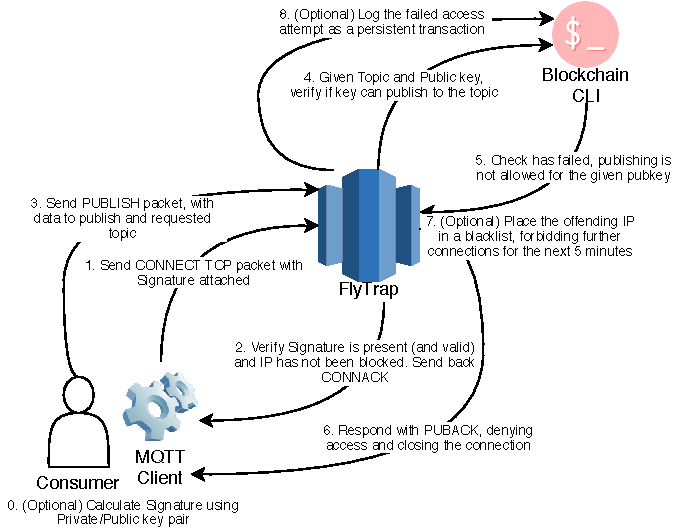
\includegraphics[width=0.9\textwidth]{workflow_fail}
    \caption{Example failed workflow to publish a message on the broker through FlyTrap}
    \label{fig:workflow_fail}
\end{figure}

\section{Consumer Layer}
First and foremost, the consumer layer. This part of the framework handles all connections between clients attempting to PUBLISH or SUBSCRIBE to data. To them, FlyTrap should be indistinguishable from a vanilla MQTT broker, which should be accepting all regular MQTT payloads. Though since every MQTT client produced in this project can connect with every MQTT Broker, a specific client is required for connection with FlyTrap - which is further explained in the section below. Moreover, an approach of identifying whether the client holds a Private Key for the presented Public Key is also needed and explained. 
\subsection{MQTT Client}
As mentioned above, FlyTrap makes use of the introduced in MQTT v5.0 User Properties\footnote{https://docs.oasis-open.org/mqtt/mqtt/v5.0/os/mqtt-v5.0-os.html\#\_Toc3901068}, allowing clients to include key-value pairs in the MQTT packets, which then can be utilised by the brokers (or other middleware). That is also where the signature and public key is being placed by the client when attempting connection with FlyTrap - and that is also the need for a custom client since regular clients are not capable of producing highly specialised signatures to connect with Ethereum blockchain.

It is important to point out, that the client is only slightly altered to provide (and compute if needed) the signature from public/private key pair. It is not a central system of the framework, as any client capable of setting User Properties for MQTT message would be sufficient, though, for the purposes of this dissertation, custom implementation has also been designed and included.
\subsection{Secure Proxy}
In order to enable FlyTrap to make decisions on whether the requests for publishing or subscribing should be accepted or denied, a secure proxy needs to be established between the clients and the MQTT Broker. As the communication between the broker and the consumers happens on Transport Layer, it is possible to insert a middleman who would be capable of inspecting the packets flowing through, dissecting it for relevant information and finally make a decision about their future journey - all without the client ever knowing that someone has intercepted the connection. 
\begin{figure}[h]
    \centering
    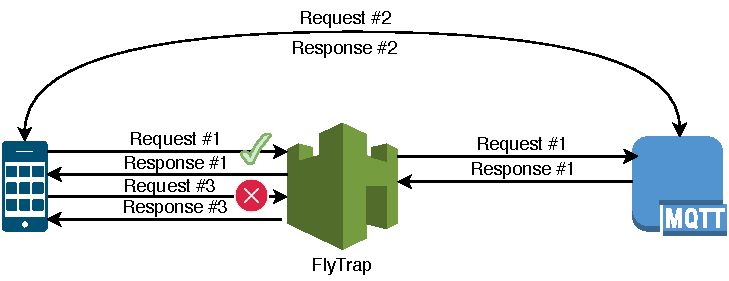
\includegraphics[width=0.8\textwidth]{tls}
    \caption{FlyTrap acting as a proxy}
    \label{fig:tls}
\end{figure}
Figure \ref{fig:tls} demonstrates all 3 possibilities when client attempts connection to a broker. In the Request \#1, FlyTrap will dissect the packet and confirm that the phone indeed can be allowed to access specific topic and then start bidirectional proxy with the broker, passing the TCP packets between two. Request \#2 shows that the same packet can be used for vanilla MQTT Broker without FlyTrap, thus decoupling the client and secure proxy, as the former can be used without the need to change the latter. Finally, for the third request, it is found that the client cannot access the requested resource and will be presented with CONACK response, with access denied flag set, terminating the connection. Though, in order to make such decisions, the proxy needs to inspect the contents of the packets.

Although this solution enough will not be sufficient, as quickly as FlyTrap can tap into the connection, the same can be assumed for potential malicious actors, which could be listening on the flowing through packets. The solution will support an extension to standard TCP - Transport Layer Security, or TLS for short, responsible for encrypting the TCP packets, significantly reducing the threat of man-in-the-middle attacks.

TLS sessions can be summarised in the following steps:
\begin{enumerate}
\item Initiate standard TCP session
\item ClientHello with client's cypher capabilities 
\item ServerHello and exchange of the cypher suite, along with server's certificate
\item Key exchange and change of cypher spec
\item Encrypted session starts
\end{enumerate}

It is vital to point out, that due to step 3 requiring server's certificate, FlyTrap will need to either obtain a copy of broker's certificates or generate a new pair, ensuring that the connecting clients will trust it. Though secure TLS connection remains optional, as it is understandable that sometimes enhanced security might cause undesirable performance losses or the MQTT broker simply does not support TLS connections - TLS will be configurable via command-line arguments.

For every new connection, a new thread (or, goroutine) is spawned which has its own context and is separated from others.

\subsection{Authenticity of public keys}
Public Keys from the Ethereum wallet are used as an identifier when determining whether a client can access a given resource or not. Though it only handles a part of the problem. Public Keys, by definition, are public, meaning that anyone could impersonate legitimate holders of the public/private key. This calls for an approach similar to the Certificate Authority problem when attempting encrypted HTTPS connections. Unfortunately, FlyTrap cannot expect every IoT device to have its own set of certificates, which would then need to be trusted by the framework in order to become recognisable - as those devices are often of limited storage and power.

In order to solve the problem of establishing whether the person presenting a public key also holds a corresponding key, signatures are used. Below you can see two figures, each outlining client-side and FlyTrap side of the signing/verification process.

\begin{figure}[h]
    \centering
    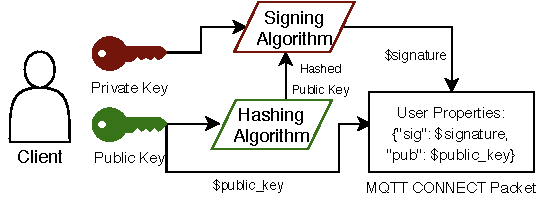
\includegraphics[width=0.8\textwidth]{sign}
    \caption{Client signing Public Key and attaching it to the message}
    \label{fig:sign}
\end{figure}

Figure \ref{fig:sign} shows how client - in possession of public/private key pair produces a signature which then is attached to the final MQTT CONNECT packet. First, it hashes the public key using Keccak-256 algorithm \cite{bertoni2009keccak} (commonly used in Ethereum, e.g. for block hashes), then it uses the private key to sign this hash and attaches obtained signature to the user properties part of the MQTT CONNECT message. Plain-text version of the public key is also attached in another field. Ethereum signatures are created by signing arbitrary bytes through a generated private key - which then can only be verified using the corresponding public key. It is also possible to extract signed bytes from the same signature in the process.

\begin{figure}[h]
    \centering
     \makebox[\textwidth][c]{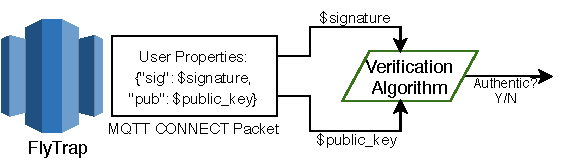
\includegraphics[width=1.1\textwidth]{verify}}
    \caption{FlyTrap verifying the signature}
    \label{fig:verify}
\end{figure}

Then, as per figure \ref{fig:verify}, FlyTrap receives the CONNECT packet and extracts both the signature \& public key from the message. As the corresponding private key for the public key was used to produce the signature, framework verifies this through Verification Algorithm. The output is a binary yes/no value - determining whether the public key was used to create the signature - along with the signed value (in this case, hashed public key) by the client. Then, framework can verify whether both signature was indeed created with the private key corresponding to the attached public key and (by hashing it again) compare the extracted value with the attached public key. This gives a definite answer that the person presenting the public key also holds the private key and thus is successfully authenticated.

For Ethereum, both Verification Algorithm and Signing Algorithm is part of Elliptic Curve Digital Signature Algorithm \citep{johnson2001elliptic}, where a public key has exactly 160 bits (which, coincidentally, is also used for ETH addresses). Hashing Algorithm - as mentioned above - is Keccak-256.
\subsection{Protecting from brute-force attacks}
Some of the failed attempts can result in a persistent log to the blockchain, which often implicates costs - primarily if FlyTrap is operating on a public blockchain. This can open a door for malicious actors attempting to drain the framework from available funds by logging many operations in a short period. Distributed Denial of Service (DDoS) attacks can also occur and overload the server, which - depending on hardware - could only handle a limited number of simultaneous connections.

To combat those problems, framework will track any failed authentication attempts in an internal dictionary, mapping IP address to the number of failed attempts. This dictionary then will be consulted whenever a new connection is initiated. If it is, then the TCP link will be shut down, and the client informed that it is currently blacklisted. Though to give the benefit of a doubt, there is a grace period of 2 prior failed attempts before a timed ban is applied. Whenever failed authentication occurs, the counter is increased by one - and if that count increases 3, the connection is terminated and dictionary updated with time 5 minutes in the future - that is the earliest time given IP can attempt the connection again.
\section{Broker Layer}

This layer is where the communication with the actual MQTT Broker occurs. Typically, it would be desirable to place both FlyTrap and the broker (e.g. Mosquitto) on the same machine (or at least the same network) to minimise the latency - though it is not necessary. Depending on the outcome of the authorisation from the Client Layer, every packet from the client is forwarded to the broker, and every packet from the broker sent back to the client. Since each connection is an individual thread, it also maintains information such as originating (\& destination) address and port - and this information will persist as long as the original connection Client <=> FlyTrap remains open - which will only be terminated if client times out, requests disconnection or for any reason authentication to FlyTrap fails.

Similar to the section discussing encrypted connection, FlyTrap is capable of either connecting with TLS-capable brokers or via plain TCP if desired (though keeping the security implications in mind, as everyone intercepting the connection would be able to read the payload).

\section{Blockchain Layer}
In this layer, communication with the Ethereum node occurs. As described in the architecture section, FlyTrap can either read or write new data onto the chain. FlyTrap should be allocated its own smart contract containing chain code capable of verifying connecting clients and relevant data structures. 
\subsection{Data model}
The root of all communication with blockchain is a smart contract that contains all chain code responsible for retrieving and storing information required by FlyTrap. Each organisation or entity willing to use FlyTrap should configure and deploy a new contract, which would be tied to a singular owner (i.e., a private key). Ethereum's chain code execution can be limited to only particular set of addresses, here most of the sensitive operations (such as adding new publishers or subscribers) are restricted to either an owner or payable ETH (set by the owner) - if the requestor is not an owner.

Then, each contract contains a single variable called ``topics'' which is a mapping (dictionary structure in Solidity, a programming language for ETH) from a string (name of the topic) to structure ``Topic'' where the metadata can be located, such as control lists. Every person can create their own topic on the contract, of which they would become the owner - this operation can be payable, if set so by the contract's owner, meaning topic creators would need to pay a fee. Figure \ref{fig:uml_topic} shows all fields used in FlyTrap's chain code placed on the blockchain, to explain further the usage and purpose of each of the fields:
\begin{figure}[h]
    \centering
    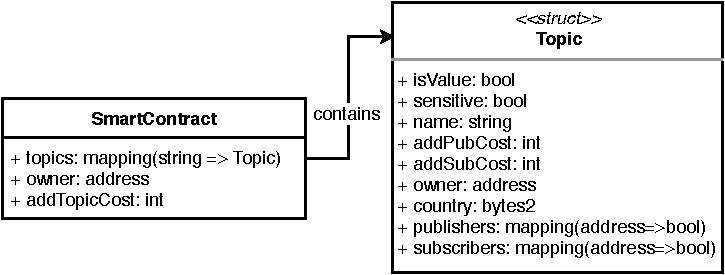
\includegraphics[width=0.9\textwidth]{uml_topic}
    \caption{Topic structure stored on blockchain}
    \label{fig:uml_topic}
\end{figure}
\begin{description}
    \item[isValue] - in Solidity, it is not possible to determine whether the given key exists in the mapping, as every value points to some arbitrary address space. An extra field helps to mitigate this issue, e.g. to avoid overwriting existing topics with new data.
    \item[sensitive] - a bool flag marking given topic as sensitive which enhances it with extra data reporting functionality outlined in section \ref{sec:reports}.
    \item[name] - a string storing topic's name, as used by the clients on the broker. It is also used as the key in the topics mapping.
    \item[addPubCost] - integer, allowing to set a price on adding new publishers to the given topic. Then, the payment will be transferred to the topic's owner.
    \item[addSubCost] - integer, similar as above, but for publishing.
    \item[owner] - ETH public address of the person that created this topic.
    \item[country] - 2-letter encoding of country to which access should be limited to for all subscribers/publishers.
    \item[publishers] - mapping from the address of a person to a true/false bool value to determine whether the given public key can publish to this topic. It is a way of creating dynamic lists in Solidity, while maintaining $O(1)$ lookup time.
    \item[subscribers] - same as above, but for subscribers.
\end{description}

Apart from base structure holding information inside the contract, events are also utilised. Event is a special structure used in Solidity, which attaches itself to the transaction log. Meaning that it is possible to append information such as user-specified reason or timestamps to all operations. This is then encoded in Application Binary Interface (ABI)\footnote{Encoding type used in Solidity: https://solidity.readthedocs.io/en/latest/abi-spec.html} JSON and sent along with the transaction. Though, it is also possible to emit empty events solely for the logging purposes \citep{dannen2017introducing}.  Figure \ref{fig:uml_event} outlines what each event consists of:
\begin{figure}[h]
    \centering
    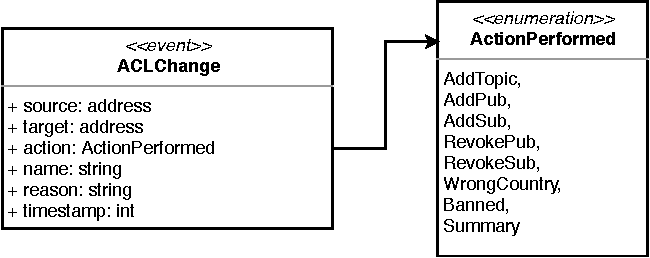
\includegraphics[width=0.8\textwidth]{uml_event}
    \caption{Event structure as stored in transaction log}
    \label{fig:uml_event}
\end{figure}

\begin{description}
    \item[source] - ETH address of the entity that caused the log to emit. E.g. for adding new topics or modifying topic's properties (such as subscribers) it is the initiators request. For system-caused logs (e.g. report summaries), it would be the contract's address.
    \item[target] - ETH address of the entity affected by the logged action. E.g. for revoking publishers/subscribers, it would be the person that's getting removed.
    \item[action] - enumeration, which defines the exact reason for the emitting the log, this can be one of the following values:
    \begin{description}
        \item[AddTopic] - when a new topic is created on the contract
        \item[AddPub] - when a new person is added as a publisher to the topic
        \item[AddSub] - when a new person is added as a subscriber to the topic
        \item[RevokePub] - when a person is removed from authorised publishers in the topic
        \item[RevokeSub] - when a person is removed from authorised subscribers in the topic
        \item[WrongCountry] - when a connection was attempted from an IP located in country that's not permitted
        \item[Banned] - when a person failed to authorise when connecting for three times in a row and was placed on a blacklist
        \item[Summary] - system-generated log for sensitive topics (see \ref{sec:reports}
    \end{description}
    \item[name] - string used to signify which topic was affected. If an action does not involve a topic, it will contain the offending IP address used to make the request.
    \item[reason] - string provided either by the user or by the system to provide further context on the action (in particular, to answer questions given by GDPR, ``why was access provisioned?'')
    \item[timestamp] - UNIX timestamp (expressed as an integer) to determine when the transaction has happened
\end{description}
\subsection{Report Generation}\label{sec:reports}
For the most sensitive topics, it is possible to enhance the security with extra measures and reporting. For every topic marked as sensitive, FlyTrap would maintain an in-memory list of all publishers or subscribers that have recently accessed the topic. Then, every specified period of time, a log will be generated and placed on blockchain that would outline all Ethereum public keys that have either published or subscribed to the given topic.

To put it in an example: if the reporting frequency is set at 30minutes and the system is started at 12:00, then client A publishes to topic  X at 12:05, and client B publishes to topic X at 12:15, finally, at 12:30 a report would be generated and placed on the blockchain which would signify that both client A \& client B published to topic X between 12:00 and 12:30. The reports should be read as follows: In the past X minutes, following public keys accessed following sensitive topics. 

It is important to consider the implications of more and less frequent reporting - since every transaction placed on a blockchain with PoW consensus algorithm has embedded gas price\footnote{Gas is a unit of work performed on Ethereum. The more complex the operation, the more gas is required, and thus more ETH currency is needed}, so the owner of the system would need to either accept the increased costs or decrease the reporting frequency. Of course, for PoA algorithms, there is no gas cost, but still, the chain code's size would grow faster in case of more frequent reporting. However, with decreased frequency, the precision also falls, so if our reporting is set to 24hrs, now we can only determine the access history in daily windows (rather than 30min ones, as shown in the example above).
\subsection{Caching operations}
Communicating with blockchain is a computationally expensive operation, and it is vital to ensure that it happens as rarely as possible in order to limit the latency caused by the security checks. Following the brute force approach, framework would issue a new request every time a connection starts - regardless whether it is part of a series of requests arriving in bulk. FlyTrap is using Ethereum as a de facto database layer, but at the same time aiming to cache the operations in-memory, which can be then quickly accessed if repeated requests occur. For checking the permissions, whenever a new request is issued, the result is stored in a map with mutex lock (to avoid race conditions).

To avoid memory filling too quickly (and eventually reaching the capabilities of the server that is running the software), the mapping used for caching will be erased every 24hrs or when the process is terminated/restarted - whichever happens first.

\subsection{Interacting with blockchain}\label{sec:interact}
As FlyTrap aims to be deployed on a publicly available blockchain, anyone can interact with the data (as long as they pay the requested fee or identify with the relevant owner's private key). For administrative operations, a simple CLI is also included, which can be called directly (not necessarily through FlyTrap) to perform administrative tasks, such as adding new topics or modifying topics restrictions.
\section{Presentation Layer}
This layer combines everything above in a front-end allowing users to inspect and interact with stored information. Similarly to section \ref{sec:interact}, this could also be read through any of the publicly available front-ends used to interact with Ethereum transactions, but to provide a complete package, the project will also ship with a simple website aiming to satisfy requirements stated in chapter 3.
\subsection{Website}
The website will not allow for writing data to blockchain (thus, does not require Ethereum wallet) which implies that all reading operations are free. Instead of using the Blockchain CLI from Blockchain Layer, the website will ship with API of its own, which will perform calls against the specific Ethereum node directly.
